\documentclass[a4paper,12pt]{article}

\usepackage[utf8x]{inputenc}
\usepackage[T2A]{fontenc}
\usepackage[english, russian]{babel}

% Опционно, требует  apt-get install scalable-cyrfonts.*
% и удаления одной строчки в cyrtimes.sty
% Сточку не удалять!
% \usepackage{cyrtimes}

% Картнки и tikz
\usepackage{graphicx}
\usepackage{tikz}
\usetikzlibrary{snakes,arrows,shapes}


% Некоторая русификация.
\usepackage{misccorr}
\usepackage{indentfirst}
\renewcommand{\labelitemi}{\normalfont\bfseries{--}}

% Увы, поля придётся уменьшить из-за листингов.
\topmargin -1cm
\oddsidemargin -0.5cm
\evensidemargin -0.5cm
\textwidth 17cm
\textheight 24cm

\sloppy

% Оглавление в PDF
\usepackage[
bookmarks=true,
colorlinks=true, linkcolor=black, anchorcolor=black, citecolor=black, menucolor=black,filecolor=black, urlcolor=black,
unicode=true
]{hyperref}

% Для исходного кода в тексте
\newcommand{\Code}[1]{\texttt{#1}}


\title{Отчёт по лабораторной работе \\ <<Динамическая IP-маршрутизация>>}
\author{(Здесь писать Ф.~И.~О)}

\begin{document}

\maketitle

\tableofcontents

\section{Настройка сети}

\subsection{Топология сети}

Топология сети и используемые IP-адреса показаны на рисунке~\ref{fig:network}.

\begin{figure}
\centering
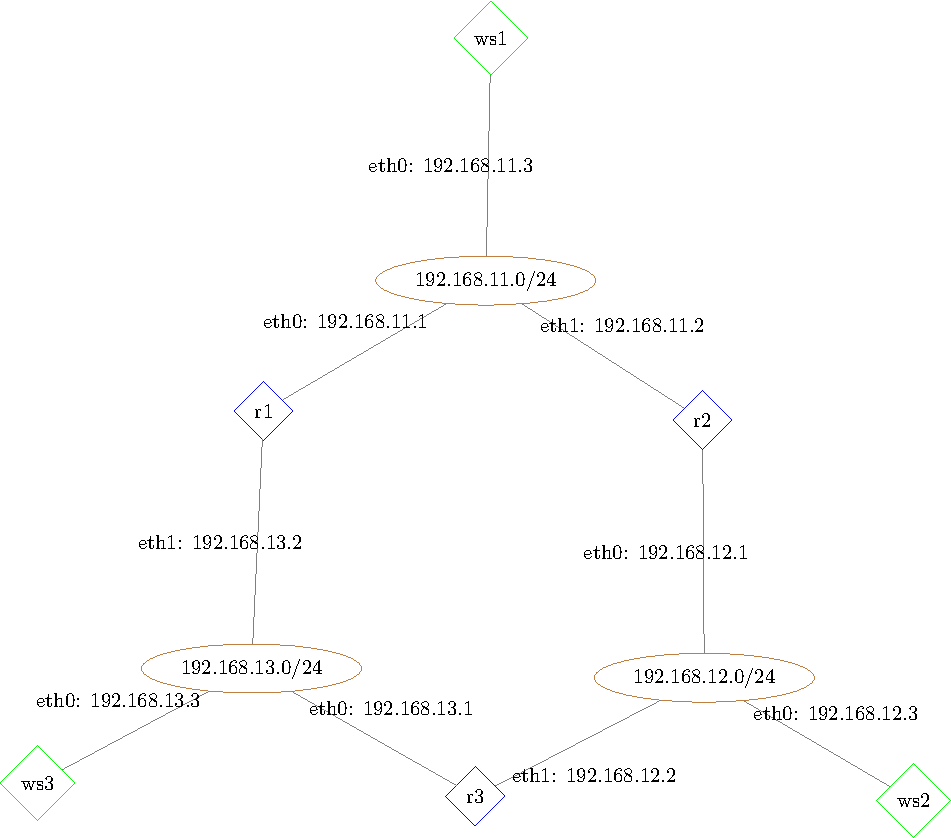
\includegraphics[width=0.8\textwidth]{includes/network_gv.pdf}
\caption{Топология сети}
\label{fig:network}
\end{figure}

Перечень узлов, на которых используется динамическая IP-маршрутизация: 
\textbf{r1}, \textbf{r2}, \textbf{r3}, \textbf{r4}, \textbf{r5}, \textbf{wsp1}


\subsection{Назначение IP-адресов}

Ниже приведён файл сетевой настройки  маршрутизатора \textbf{r1}:

\begin{Verbatim}
auto lo
iface lo inet loopback

auto eth0
iface eth0 inet static
address 10.103.0.1
netmask 255.255.0.0

auto eth1
iface eth1 inet static
address 10.104.0.1
netmask 255.255.0.0
\end{Verbatim}

Ниже приведён файл сетевой настройки  маршрутизатора \textbf{r2}:

\begin{Verbatim}
auto lo
iface lo inet loopback

auto eth0
iface eth0 inet static
address 10.102.0.1
netmask 255.255.0.0

auto eth1
iface eth1 inet static
address 10.103.0.2
netmask 255.255.0.0
\end{Verbatim}

Ниже приведён файл сетевой настройки  маршрутизатора \textbf{r3}:

\begin{Verbatim}
auto lo
iface lo inet loopback

auto eth0
iface eth0 inet static
address 10.101.0.1
netmask 255.255.0.0

auto eth1
iface eth1 inet static
address 10.102.0.2
netmask 255.255.0.0

auto eth2
iface eth2 inet static
address 10.106.0.1
netmask 255.255.0.0
\end{Verbatim}

Ниже приведён файл сетевой настройки  маршрутизатора \textbf{r4}:

\begin{Verbatim}
auto lo
iface lo inet loopback

auto eth0
iface eth0 inet static
address 10.103.0.3
netmask 255.255.0.0

auto eth1
iface eth1 inet static
address 10.105.0.1
netmask 255.255.0.0

auto eth2
iface eth2 inet static
address 10.106.0.2
netmask 255.255.0.0
\end{Verbatim}

Ниже приведён файл сетевой настройки  маршрутизатора \textbf{r5}:

\begin{Verbatim}
auto lo
iface lo inet loopback

auto eth0
iface eth0 inet static
address 10.104.0.2
netmask 255.255.0.0

auto eth1
iface eth1 inet static
address 10.105.0.2
netmask 255.255.0.0
\end{Verbatim}

Ниже приведён файл сетевой настройки рабочей станции \textbf{ws1}:

\begin{Verbatim}
auto lo
iface lo inet loopback

auto eth0
iface eth0 inet static
address 10.101.0.2
netmask 255.255.0.0
\end{Verbatim}

Ниже приведён файл сетевой настройки рабочей станции \textbf{wsp1}:

\begin{Verbatim}
auto lo
iface lo inet loopback

auto eth0
iface eth0 inet static
address 10.103.0.4
netmask 255.255.0.0
\end{Verbatim}


\subsection{Настройка протокола RIP}

Ниже приведен файл \Code{/etc/quagga/ripd.conf} маршрутизатора \textbf{r1}:

\begin{Verbatim}
router rip

network eth0
network eth1

timers basic 10 60 120

redistribute kernel
redistribute connected

log file /var/log/quagga/ripd.log
\end{Verbatim}

Ниже приведен файл \Code{/etc/quagga/ripd.conf} маршрутизатора \textbf{r2}:

\begin{Verbatim}
router rip

network eth0
network eth1

timers basic 10 60 120

redistribute kernel
redistribute connected

log file /var/log/quagga/ripd.log
\end{Verbatim}

Ниже приведен файл \Code{/etc/quagga/ripd.conf} маршрутизатора \textbf{r3}:

\begin{Verbatim}
router rip

network eth1
network eth2

timers basic 10 60 120

redistribute kernel
redistribute connected

log file /var/log/quagga/ripd.log
\end{Verbatim}

Ниже приведен файл \Code{/etc/quagga/ripd.conf} маршрутизатора \textbf{r4}:

\begin{Verbatim}
router rip

network eth0
network eth1
network eth2

timers basic 10 60 120

redistribute kernel
redistribute connected

log file /var/log/quagga/ripd.log
\end{Verbatim}

Ниже приведен файл \Code{/etc/quagga/ripd.conf} маршрутизатора \textbf{r5}:

\begin{Verbatim}
router rip

network eth0
network eth1

timers basic 10 60 120

redistribute kernel
redistribute connected

log file /var/log/quagga/ripd.log
\end{Verbatim}

Ниже приведен файл \Code{/etc/quagga/ripd.conf} рабочий станции, связанной с несколькими маршрутизаторами \textbf{wsp1}.

\begin{Verbatim}
router rip

network eth0

timers basic 10 60 120

redistribute kernel
redistribute connected

log file /var/log/quagga/ripd.log
\end{Verbatim}


\section{Проверка настройки протокола RIP}

Вывод \textbf{traceroute} от узла такого-то до такого-то при нормальной работе сети.

\begin{Verbatim}
Сюда нужно поместить вывод traceroute.
\end{Verbatim}

Вывод \textbf{traceroute} от узла такого-то до внешнего IP (195.19.38.2 сгодится).

\begin{Verbatim}
Сюда нужно поместить вывод traceroute.
\end{Verbatim}

Вывод сообщения RIP.

\begin{Verbatim}
Перехваченное сообщение RIP от любого маршрутизатора
\end{Verbatim}

Вывод таблицы RIP.

\begin{Verbatim}
Таблица RIP
\end{Verbatim}

Вывод таблицы маршрутизации.

\begin{Verbatim}
Таблица маршрутизации
\end{Verbatim}

\section{Расщепленный горизонт и испорченные обратные обновления}

Поместить сюда вывод сообщения одного и того же маршрутизатор с включенным расщ. горизонтом, с включенными испорченными обновлениями, с отключённым расщ. гор.

Объяснить разницу.

Вернуть настройки в исходное состояние (включенный без испорченных).

\section{Имитация устранимой поломки в сети}

Какой маршрутизатор выключили?

Вывод таблицы RIP непосредственно перед истечением таймера устаревания (на маршрутизаторе-соседе отключенного).

\begin{Verbatim}
Таблица RIP
\end{Verbatim}

Перестроенная таблица на этом же маршрутизаторе

\begin{Verbatim}
Таблица RIP
\end{Verbatim}


Вывод \textbf{traceroute} от узла такого-то до такого-то после того, как служба RIP перестроила таблицы маршрутизации.

\begin{Verbatim}
Сюда нужно поместить вывод traceroute после "поломки".
\end{Verbatim}

\section{Имитация неустранимой поломки в сети}

Какой маршрутизатор выключили? (Теперь у нас нет связанной сети)

Далее поместить таблицы протокола RIP, где видна 16-ая метрика, и сообщения протокола RIP с 16-ой метрикой.

\end{document}
